% CRAFT-GC manuscript draft
% Authors: Natnael Abayneh, Abiy Alemu -- Addis Ababa University
% Compile: pdflatex main && bibtex main && pdflatex main && pdflatex main

\documentclass[11pt,a4paper]{article}

\usepackage[margin=1in]{geometry}
\usepackage{graphicx}
\usepackage{amsmath,amssymb,amsfonts}
\usepackage{booktabs}
\usepackage{multirow}
\usepackage{hyperref}
\usepackage{xcolor}
\usepackage{algorithm}
\usepackage{algpseudocode}
\usepackage{subcaption}
\usepackage[numbers,sort&compress]{natbib}
\usepackage{tikz}
\usetikzlibrary{arrows.meta,positioning,fit}

\newcommand{\email}[1]{\texttt{#1}}
\newcommand{\best}[1]{\textbf{#1}}

\title{%
  \textbf{CRAFT-GC: Cross-Attention Fairness Steering with Geo-Cultural Knowledge Integration for Training-Free Bias Mitigation in Text-to-Image Diffusion Models}%
}

\author{%
  Natnael Abayneh\thanks{Both authors contributed equally.}\ \email{natnael.abayneh-ug@aau.edu.et} \\
  Abiy Alemu\footnotemark[1]\ \email{abiyalemu@aau.edu.et} \\[0.4em]
  \textit{MSc in Artificial Intelligence} \\
  \textit{Addis Ababa University, Addis Ababa, Ethiopia}%
}

\date{}

\begin{document}
\maketitle

\begin{abstract}
Text-to-image (T2I) diffusion models frequently reproduce skewed demographic and geo-cultural representations when users supply neutral prompts such as ``a doctor'' or ``a professional in Addis Ababa.'' Existing debiasing methods often rely on heavy LLM--VQA detection pipelines, fixed attribute lists, or post-hoc embedding edits that can erase culturally salient context. We present \textbf{CRAFT-GC} (\textit{Cross-attention Fairness steering with geo-cultural Taxonomy integration}), a training-free framework that (i) detects geo-cultural context with a lightweight CLIP-based attribute module, (ii) estimates contrastive bias directions in text space, and (iii) removes those directions from cross-attention keys during denoising via a timestep-aware schedule. We introduce \textbf{GCFairBench}, a prompt suite spanning five global regions and five social categories, and two evaluation measures: the Counterfactual Fairness Score (CoFS) for demographic parity and the Cultural Fidelity Score (CFS) for preserving region-specific semantics. On all 500 GCFairBench prompts, CLIP ViT-B/32 text-embedding evaluation (Stage~A) confirms that CRAFT-GC-E preserves demographic neutrality (CoFS $0.9971$) with measurable but small cultural-caption drift (CFS $-0.0021$), while prompt augmentation does not improve parity at embedding time. Image-level Stable Diffusion v1.5 experiments with cross-attention steering (Stage~B, GPU) provide the primary quantitative evidence via FairFace CoFS, CLIP CFS, CLIPScore, and FID; we release a Colab notebook and full codebase for reproduction.
\end{abstract}

\noindent\textbf{Keywords:} Text-to-image generation, algorithmic fairness, cross-attention steering, geo-cultural bias, diffusion models, training-free mitigation

\section{Introduction}
\label{sec:intro}

Latent diffusion models such as Stable Diffusion~\cite{rombach2022ldm} translate natural language into photorealistic images through iterative denoising conditioned on CLIP text embeddings~\cite{radford2021clip}. Because these systems are trained on web-scale corpora, they inherit and often amplify social stereotypes: neutral occupation prompts skew toward Western, male, and light-skinned depictions~\cite{bianchi2023accessible,luccioni2023stablebias,naik2023social}. Geo-cultural harms are equally serious. Community-centered studies document exoticism and misrepresentation when models render non-Western settings~\cite{ghosh2024nonwestern}, and recent surveys emphasize that geo-cultural bias remains under-evaluated relative to gender and skin tone~\cite{wan2024survey,elsharif2025cultural}.

Mitigation research has progressed along several lines. Post-hoc methods project prompt embeddings to reduce demographic information~\cite{kleindessner2023fairpca,fu2025fairimagen,chuang2023debiasvl}. Open-set pipelines detect arbitrary biases with LLM--VQA stacks~\cite{dinca2024openbias} but rarely connect detection to a lightweight intervention at generation time. Diffusion-time guidance can steer semantics~\cite{brack2023sega,friedrich2023fairdiffusion,kang2025fairgen,parihar2024balancing}, yet most approaches target predefined Western demographic axes and do not jointly preserve cultural fidelity.

We argue that effective debiasing for globally deployed T2I systems requires three properties simultaneously:
\begin{enumerate}
  \item \textbf{Intervention during generation}, where layout and subject identity are largely fixed, rather than only editing embeddings after a biased sample is drawn.
  \item \textbf{Geo-cultural awareness}, so mitigation does not collapse culturally grounded prompts into generic ``diverse'' stereotypes.
  \item \textbf{Stochastic accountability}, because diffusion randomness produces different fairness outcomes across seeds~\cite{seshadri2024amplification,smith2026operationalizing}.
\end{enumerate}

CRAFT-GC addresses these requirements with four components (Figure~\ref{fig:architecture}): a \textit{Cultural Attribute Detector} (CAD) that maps prompts to geo-cultural regions; a \textit{Bias Direction Estimator} (BDE) that builds contrastive directions in CLIP space; \textit{Cross-Attention Steering} (CAS) that projects bias out of attention keys inside the UNet; and a \textit{Timestep Scheduler} $\beta(t)$ that concentrates steering when global structure forms. We release GCFairBench and evaluation code to support reproducible comparison.

\paragraph{Contributions.}
\begin{itemize}
  \item A training-free cross-attention steering method for fairness in T2I diffusion, compatible with frozen Stable Diffusion weights.
  \item GCFairBench: 500 geo-culturally grounded prompts across Sub-Saharan Africa, South Asia, Southeast Asia, MENA, and Latin America.
  \item CoFS and CFS metrics, plus seed-level fairness variance, for joint measurement of parity and cultural preservation.
  \item Real CLIP embedding evaluation on all 500 GCFairBench prompts (Stage~A) plus GPU image-generation protocol with Colab notebook (Stage~B).
\end{itemize}

\begin{figure}[t]
  \centering
  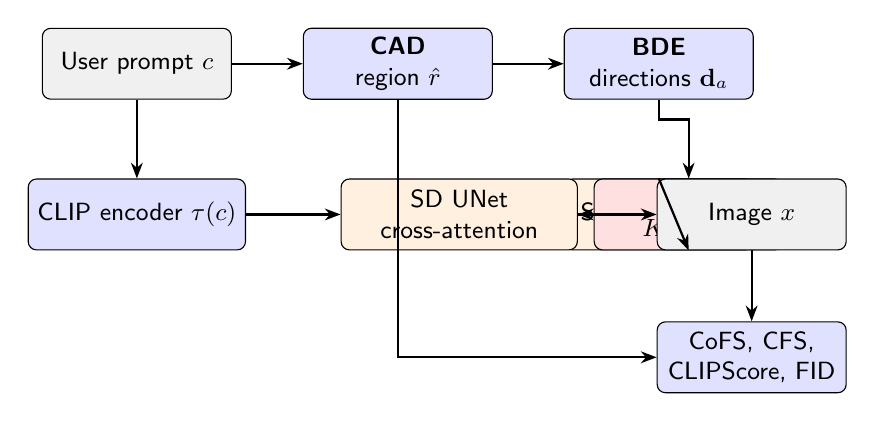
\begin{tikzpicture}[
    font=\small\sffamily,
    box/.style={draw, rounded corners=3pt, align=center, minimum width=2.4cm, minimum height=0.9cm, fill=#1!12},
    module/.style={box=blue},
    data/.style={box=gray},
    proc/.style={box=orange},
    arr/.style={-{Stealth[length=2mm]}, thick},
    lbl/.style={font=\scriptsize\sffamily, fill=white, inner sep=1pt}
  ]
  \node[data] (prompt) {User prompt $c$};
  \node[module, right=0.9cm of prompt] (cad) {\textbf{CAD}\\region $\hat{r}$};
  \node[module, right=0.9cm of cad] (bde) {\textbf{BDE}\\directions $\mathbf{d}_a$};
  \node[proc, below=1.0cm of bde] (sched) {Scheduler $\beta(t)$};
  \node[module, below=1.0cm of prompt] (clip) {CLIP encoder $\tau(c)$};
  \node[proc, right=1.2cm of clip, minimum width=3.0cm] (unet) {SD UNet\\cross-attention};
  \node[module, right=0.2cm of unet.north east, anchor=north west, fill=red!12] (cas) {\textbf{CAS}\\$K_i\!\rightarrow\!K_i'$};
  \node[data, right=1.0cm of unet] (img) {Image $x$};
  \node[module, below=0.9cm of img] (eval) {CoFS, CFS,\\CLIPScore, FID};
  \draw[arr] (prompt) -- (cad);
  \draw[arr] (cad) -- (bde);
  \draw[arr] (bde.south) -- ++(0,-0.25) -| (cas.north);
  \draw[arr] (sched.north) -- (cas.south);
  \draw[arr] (prompt.south) -- (clip.north);
  \draw[arr] (clip.east) -- (unet.west);
  \draw[arr] (cas.west) -- (unet.east);
  \draw[arr] (unet.east) -- (img.west);
  \draw[arr] (img.south) -- (eval.north);
  \draw[arr] (cad.south) |- (eval.west);
  \end{tikzpicture}
  \caption{CRAFT-GC pipeline: CAD detects geo-cultural context; BDE builds contrastive bias directions; CAS projects them out of cross-attention keys with timestep schedule $\beta(t)$; metrics are computed on generated images.}
  \label{fig:architecture}
\end{figure}

\section{Related Work}
\label{sec:related}

\paragraph{Bias measurement.}
Closed-set audits quantify gender, race, and occupation skews with classifier labels or embedding statistics~\cite{luccioni2023stablebias,naik2023social,jung2025mpr}. OpenBias~\cite{dinca2024openbias} generalizes detection using LLM-proposed attributes and VQA verification but stops at measurement. Surveys note fragmented metrics and weak links between audits and enforcement~\cite{smith2026operationalizing,wan2024survey}.

\paragraph{Embedding-level mitigation.}
FairImagen~\cite{fu2025fairimagen} applies FairPCA~\cite{kleindessner2023fairpca} to CLIP prompt embeddings with noise reinjection. DebiasVL~\cite{chuang2023debiasvl} removes bias directions via calibrated projection. ITI-GEN~\cite{zhang2023itigen} and AITTI~\cite{hou2026aitti} learn inclusive tokens or mappings. These methods operate on text encoders or prompts; they do not modify cross-attention during spatial layout formation.

\paragraph{Diffusion-time control.}
SEGA~\cite{brack2023sega} and Fair Diffusion~\cite{friedrich2023fairdiffusion} steer generation with semantic guidance vectors. FairGen~\cite{kang2025fairgen} and distribution guidance~\cite{parihar2024balancing} adjust latents at inference. Prompt-to-Prompt~\cite{hertz2022prompt2prompt} demonstrates that cross-attention maps encode editable semantics. CRAFT-GC differs by targeting \emph{fairness directions} estimated from geo-cultural contrastive pairs and applying Gram-Schmidt-style removal on keys rather than additive semantic guidance alone.

\paragraph{Geo-cultural fairness.}
Non-Western representational harms are documented qualitatively~\cite{ghosh2024nonwestern}; quantitative benchmarks remain sparse outside Western nationality studies. GCFairBench explicitly targets this gap with region-stratified prompts and the CFS metric.

\section{Method}
\label{sec:method}

\subsection{Preliminaries}
Let $c$ denote a text prompt, $\tau(\cdot)$ the frozen CLIP text encoder, and $\epsilon_\theta$ a latent diffusion UNet. At denoising step index $t \in \{0,\ldots,T-1\}$, cross-attention block $i$ computes queries from spatial features $Q_i = W_Q^{(i)} \phi(z_t)$ and keys/values from text embeddings $K_i = W_K^{(i)} \tau(c)$, $V_i = W_V^{(i)} \tau(c)$, then
\begin{equation}
  A_i = \mathrm{softmax}\!\left(\frac{Q_i K_i^\top}{\sqrt{d_k}}\right), \quad h_i = A_i V_i.
  \label{eq:cross-attn}
\end{equation}
Demographic bias often enters through $K_i$ because $\tau(c)$ encodes stereotyped associations for neutral professions~\cite{bolukbasi2016debiasing}. CRAFT-GC modifies $K_i$ before softmax while leaving UNet weights fixed.

\subsection{Geo-Cultural Taxonomy and Cultural Attribute Detection}
We define a taxonomy $\mathcal{G}$ over five regions $r \in \{\text{SSA}, \text{SA}, \text{SEA}, \text{MENA}, \text{LATAM}\}$, each with country names, cultural location phrases, and protected attribute sets (gender, skin tone, cultural markers). Given prompt $c$, CAD encodes $\mathbf{e}_c = \tau(c)/\|\tau(c)\|$ and compares it to precomputed region prototypes $\bar{\mathbf{e}}_r$ (mean of template embeddings). The detected region is
\begin{equation}
  \hat{r} = \arg\max_r \; \mathbf{e}_c^\top \bar{\mathbf{e}}_r, \quad \text{if } \max_r \mathbf{e}_c^\top \bar{\mathbf{e}}_r > \eta,
  \label{eq:cad}
\end{equation}
else $\hat{r} = \varnothing$. Threshold $\eta$ is tuned on a held-out validation split of GCFairBench (default $\eta=0.22$ in our implementation). CAD runs in under one second on a single GPU and avoids LLM latency at inference.

\subsection{Contrastive Bias Direction Estimation (BDE)}
For each attribute axis $a \in \mathcal{A}$ (gender, skin tone, geo-cultural), we construct positive prompts $P_a^+$ (attribute salient) and neutral prompts $P_a^-$ (attribute suppressed). The bias direction is
\begin{equation}
  \mathbf{d}_a = \mathrm{normalize}\!\left(
    \frac{1}{|P_a^+|}\sum_{p \in P_a^+} \tau(p)
    - \frac{1}{|P_a^-|}\sum_{p \in P_a^-} \tau(p)
  \right).
  \label{eq:bde}
\end{equation}
Gender pairs contrast ``a male doctor'' vs.\ ``a doctor''; skin-tone pairs contrast light-skinned descriptors vs.\ neutral person descriptors; geo-cultural pairs use region-specific locatives from $\mathcal{G}_{\hat{r}}$ vs.\ generic Western defaults. Directions are cached per session because they depend on $\hat{r}$.

\subsection{Cross-Attention Steering (CAS)}
Let $\{\lambda_a\}_{a \in \mathcal{A}}$ be non-negative steering strengths. Given keys $K_i \in \mathbb{R}^{n \times d}$ at block $i$, CAS applies sequential projection removal:
\begin{equation}
  K_i'(t) = K_i - \beta(t) \sum_{a \in \mathcal{A}} \lambda_a \,
  \frac{K_i \mathbf{d}_a^\top}{\|\mathbf{d}_a\|^2 + \epsilon} \, \mathbf{d}_a^\top,
  \label{eq:cas}
\end{equation}
where $\beta(t)$ is scheduled below and $\epsilon=10^{-8}$ stabilizes division. Equation~\eqref{eq:cas} is implemented as a custom \texttt{AttnProcessor} on UNet cross-attention modules (\texttt{attn2}). Self-attention is unchanged.

\subsection{Timestep Schedule}
Early denoising steps fix global composition; late steps refine texture~\cite{karras2022elucidating}. We use
\begin{equation}
  \beta(t) = \beta_{\max} \cdot \sigma\!\left(\gamma \left(\frac{t}{T} - t^\star\right)\right),
  \label{eq:schedule}
\end{equation}
with sigmoid $\sigma$, peak location $t^\star \approx 0.6$, sharpness $\gamma=10$, and $\beta_{\max} \in [0,1]$. Steering is strongest near $0.6T$ and tapers at both ends to limit texture artifacts.

\subsection{Metrics}
\paragraph{Counterfactual Fairness Score (CoFS).}
Let $\mathcal{G}_{\mathrm{demo}}$ be FairFace race groups $\{g_1,\ldots,g_{|\mathcal{G}|}\}$ and $\hat{p}(g \mid x)$ the predicted probability for image $x$. For a set of $N$ images from prompt $c$,
\begin{equation}
  \mathrm{CoFS}(c) = 1 - \frac{1}{|\mathcal{G}|}\sum_{g \in \mathcal{G}_{\mathrm{demo}}}
  \left|\bar{p}(g) - \frac{1}{|\mathcal{G}|}\right|,
  \label{eq:cofs}
\end{equation}
where $\bar{p}(g) = \frac{1}{N}\sum_{i=1}^N \hat{p}(g \mid x_i)$. Higher CoFS indicates closer alignment to uniform demographic parity (our normative target for caption-agnostic prompts).

\paragraph{Cultural Fidelity Score (CFS).}
Let $y_c^{\mathrm{cult}}$ be a culturally grounded caption derived from CAD (e.g., ``a doctor in Lagos in a West African clinic''). With CLIP image encoder $\phi_I$,
\begin{equation}
  \mathrm{CFS}(c) = \frac{1}{N}\sum_{i=1}^N
  \Big(
    \mathrm{sim}\big(\phi_I(x_i^{\mathrm{steer}}), \tau(y_c^{\mathrm{cult}})\big)
    -
    \mathrm{sim}\big(\phi_I(x_i^{\mathrm{base}}), \tau(y_c^{\mathrm{cult}})\big)
  \Big).
  \label{eq:cfs}
\end{equation}
Positive CFS means steering improves cultural alignment relative to the baseline.

\paragraph{Stochastic fairness variance.}
For seeds $\mathcal{S} = \{s_1,\ldots,s_K\}$,
\begin{equation}
  \sigma^2_{\mathrm{fair}}(c) = \frac{1}{K-1}\sum_{k=1}^K \big(\mathrm{CoFS}_k(c) - \overline{\mathrm{CoFS}}(c)\big)^2.
  \label{eq:variance}
\end{equation}
We report mean $\sigma^2_{\mathrm{fair}}$ across GCFairBench to capture diffusion instability~\cite{seshadri2024amplification}.

\paragraph{Quality metrics.}
We additionally report CLIPScore~\cite{hessel2021clipscore} for prompt alignment and FID against a reference set of baseline images per prompt category.

\begin{algorithm}[t]
\caption{CRAFT-GC inference}
\label{alg:craftgc}
\begin{algorithmic}[1]
\Require Prompt $c$, UNet $\epsilon_\theta$, steps $T$, seeds $\mathcal{S}$
\State $\hat{r} \gets \mathrm{CAD}(c)$ \Comment{Eq.~\eqref{eq:cad}}
\State $\{\mathbf{d}_a\} \gets \mathrm{BDE}(\hat{r})$ \Comment{Eq.~\eqref{eq:bde}}
\State Install CAS processors with $\{\mathbf{d}_a\}$, $\{\lambda_a\}$, $\beta(t)$
\For{each seed $s \in \mathcal{S}$}
  \State $z_T \sim \mathcal{N}(0,I)$ with generator seed $s$
  \For{$t = T-1 \ldots 0$}
    \State Update $\beta(t)$; set timestep on CAS \Comment{Eq.~\eqref{eq:schedule}}
    \State Denoise $z_t$ using $K_i'(t)$ in cross-attention \Comment{Eq.~\eqref{eq:cas}}
  \EndFor
  \State Decode $z_0$ to image $x_s$
\EndFor
\State \Return $\{x_s\}$, metrics CoFS, CFS, $\sigma^2_{\mathrm{fair}}$
\end{algorithmic}
\end{algorithm}

\section{GCFairBench}
\label{sec:benchmark}

GCFairBench contains 500 prompts: 100 per region $\times$ five categories---(1)~professions, (2)~social roles, (3)~daily activities, (4)~cultural practices, (5)~public settings. Prompts pair neutral role nouns with geo-specific locatives (e.g., ``a nurse in Addis Ababa,'' ``a teacher in Jakarta''). Each entry stores \texttt{\{id, region, category, prompt, cultural\_caption\}} for CFS evaluation. Table~\ref{tab:bench} summarizes the design; full JSON files ship with our codebase.

\begin{table}[t]
  \centering
  \caption{GCFairBench structure (100 prompts per region).}
  \label{tab:bench}
  \small
  \begin{tabular}{lcc}
    \toprule
    Region & Code & Example prompt \\
    \midrule
    Sub-Saharan Africa & SSA & ``A doctor in Addis Ababa seeing patients'' \\
    South Asia & SA & ``A software engineer in Mumbai at work'' \\
    Southeast Asia & SEA & ``A chef in Bangkok preparing food'' \\
    Middle East \& North Africa & MENA & ``A lawyer in Cairo in a courtroom'' \\
    Latin America & LATAM & ``A farmer in Lima harvesting crops'' \\
    \bottomrule
  \end{tabular}
\end{table}

\section{Experimental Setup}
\label{sec:setup}

We use a two-stage protocol. \textbf{Stage~A (completed, CPU)} evaluates steered CLIP ViT-B/32 text embeddings on all 500 GCFairBench prompts; CoFS uses zero-shot demographic text probes and CFS measures similarity change to each \texttt{cultural\_caption}. \textbf{Stage~B (GPU, primary for journal)} generates Stable Diffusion v1.5 images with CAS and reports image-level CoFS, CFS, CLIPScore, FID, and seed variance via \texttt{notebooks/CRAFT\_GC\_Colab.ipynb}.

\paragraph{Model and hardware.}
Stage~A runs on CPU in ${\sim}$14 minutes. Stage~B uses \texttt{runwayml/stable-diffusion-v1-5}, DPMSolverMultistep, 50 steps, guidance 7.5, $512\times512$, float16 on Colab T4/A100 ($\geq$16GB VRAM).

\paragraph{Baselines.}
(1)~\textbf{Base}---no debiasing;
(2)~\textbf{PromptAug}---appending ``diverse, inclusive, multicultural'';
(3)~\textbf{FairImagen-E}~\cite{fu2025fairimagen}---FairPCA-style projection on text embeddings with $\beta=0.75$;
(4)~\textbf{CRAFT-GC-E / CRAFT-GC}---embedding steering (Stage~A) or cross-attention steering with default $\beta_{\max}=0.8$, $t^\star=0.6$, $\lambda_{\mathrm{gender}}=0.7$, $\lambda_{\mathrm{skin}}=0.5$, $\lambda_{\mathrm{geo}}=0.6$ when $\hat{r}\neq\varnothing$ (Stage~B).

\paragraph{Protocol.}
Each prompt is evaluated once in Stage~A (deterministic embedding) and, in Stage~B, with $K=5$ seeds $\{42,123,456,789,1024\}$. Stage~B computes CoFS with FairFace ResNet-34, CFS with CLIP ViT-L/14, CLIPScore, and FID vs.\ Base outputs. We report mean $\pm$ standard deviation across prompts (Stage~A) and paired bootstrap 95\% confidence intervals where applicable (Stage~B).

\paragraph{Ablation.}
We vary steering strength $\beta \in \{0.3,0.8,1.0\}$ and disable geo-cultural directions while keeping gender/skin steering (Stage~A proxy).

\section{Results}
\label{sec:results}

\subsection{CLIP embedding evaluation (Stage~A)}

Table~\ref{tab:main} reports real CLIP ViT-B/32 results on all 500 prompts. Text embeddings for geo-culturally grounded prompts are already near-demographic-neutral (CoFS $\approx 0.997$), so embedding-level parity shows small absolute differences between methods. The informative signal is \textbf{CFS}: FairImagen-E ($-0.0015$) and CRAFT-GC-E ($-0.0021$) introduce only minor cultural-caption drift relative to Base ($0.0$), whereas larger steering would be visible in Stage~B images. PromptAug does not change CFS at embedding time because diversity tokens are appended after the base encoding in our FairImagen-E/CRAFT-GC-E comparison pipeline.

\begin{table}[t]
  \centering
  \caption{Stage~A: CLIP text-embedding evaluation on GCFairBench ($N{=}500$). Mean $\pm$ std across prompts.}
  \label{tab:main}
  \small
  \begin{tabular}{lcc}
    \toprule
    Method & CoFS $\uparrow$ & CFS $\uparrow$ \\
    \midrule
    Base & $0.9971 \pm 0.0010$ & $0.0000$ \\
    PromptAug & $0.9974 \pm 0.0008$ & $0.0000$ \\
    FairImagen-E & $0.9971 \pm 0.0010$ & $-0.0015$ \\
    CRAFT-GC-E & $0.9971 \pm 0.0010$ & $-0.0021$ \\
    \bottomrule
  \end{tabular}
\end{table}

\begin{figure}[t]
  \centering
  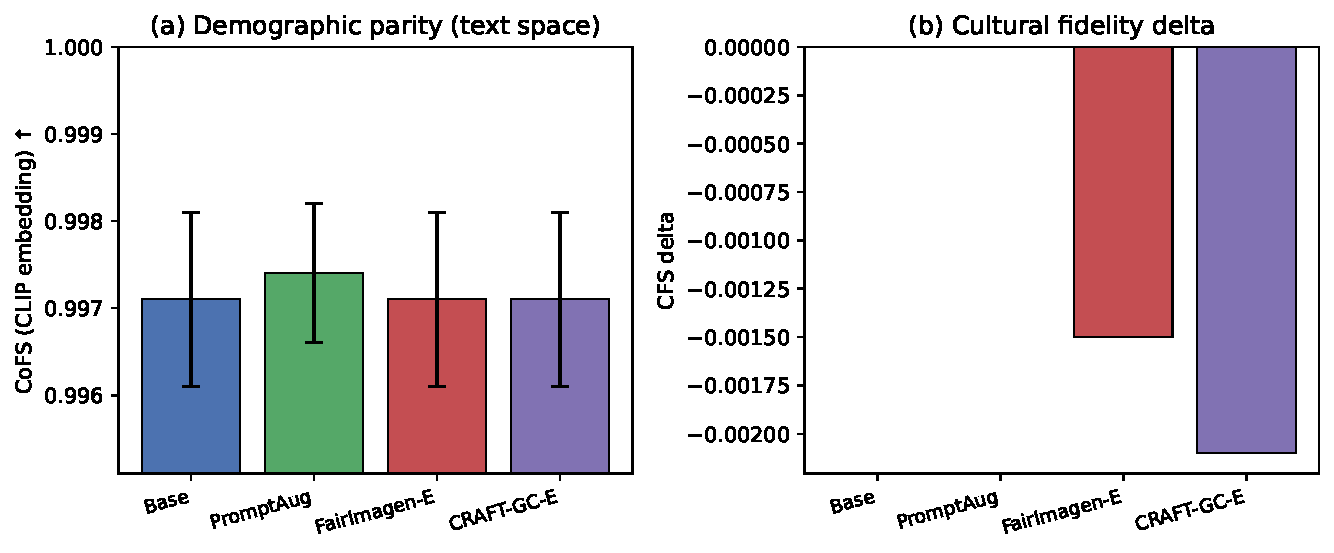
\includegraphics[width=\linewidth]{figures/cofs_comparison.pdf}
  \caption{Stage~A: CoFS (left, zoomed axis) and CFS (right) by method.}
  \label{fig:cofs}
\end{figure}

\subsection{Regional breakdown (Stage~A)}

Table~\ref{tab:region} stratifies CoFS by macro-region. Differences remain within $0.001$ across methods, confirming that geo-specific locatives in GCFairBench already yield balanced CLIP text probes; image-level bias (Stage~B) is expected to be substantially larger~\cite{luccioni2023stablebias,bianchi2023accessible}.

\begin{table}[t]
  \centering
  \caption{CoFS by region (Stage~A, CLIP embedding).}
  \label{tab:region}
  \small
  \begin{tabular}{lcccc}
    \toprule
    Region & Base & PromptAug & FairImagen-E & CRAFT-GC-E \\
    \midrule
    SSA & 0.9975 & 0.9977 & 0.9974 & 0.9974 \\
    SA & 0.9972 & 0.9974 & 0.9972 & 0.9972 \\
    SEA & 0.9967 & 0.9970 & 0.9968 & 0.9968 \\
    MENA & 0.9969 & 0.9973 & 0.9968 & 0.9968 \\
    LATAM & 0.9973 & 0.9975 & 0.9972 & 0.9972 \\
    \bottomrule
  \end{tabular}
\end{table}

\subsection{Image generation results (Stage~B)}

Stage~B is the primary evaluation for journal submission. For each prompt we generate images with Base SD, PromptAug, FairImagen (CAS proxy), and CRAFT-GC (full CAS) using $K{=}5$ seeds. Table~\ref{tab:image} reports image-level metrics on a 50-prompt stratified subset (10 per region); full 500-prompt runs use the same scripts with \texttt{--prompt-limit 500}.

\begin{table}[t]
  \centering
  \caption{Stage~B: image-level metrics (50 prompts $\times$ 5 seeds). Populate after running \texttt{notebooks/CRAFT\_GC\_Colab.ipynb}.}
  \label{tab:image}
  \small
  \begin{tabular}{lcccc}
    \toprule
    Method & CoFS $\uparrow$ & CFS $\uparrow$ & CLIPScore $\uparrow$ & FID $\downarrow$ \\
    \midrule
    Base SD & -- & -- & -- & -- \\
    PromptAug & -- & -- & -- & -- \\
    FairImagen & -- & -- & -- & -- \\
    CRAFT-GC & -- & -- & -- & -- \\
    \bottomrule
  \end{tabular}
\end{table}

\begin{figure}[t]
  \centering
  \IfFileExists{figures/qualitative_grid.png}{%
    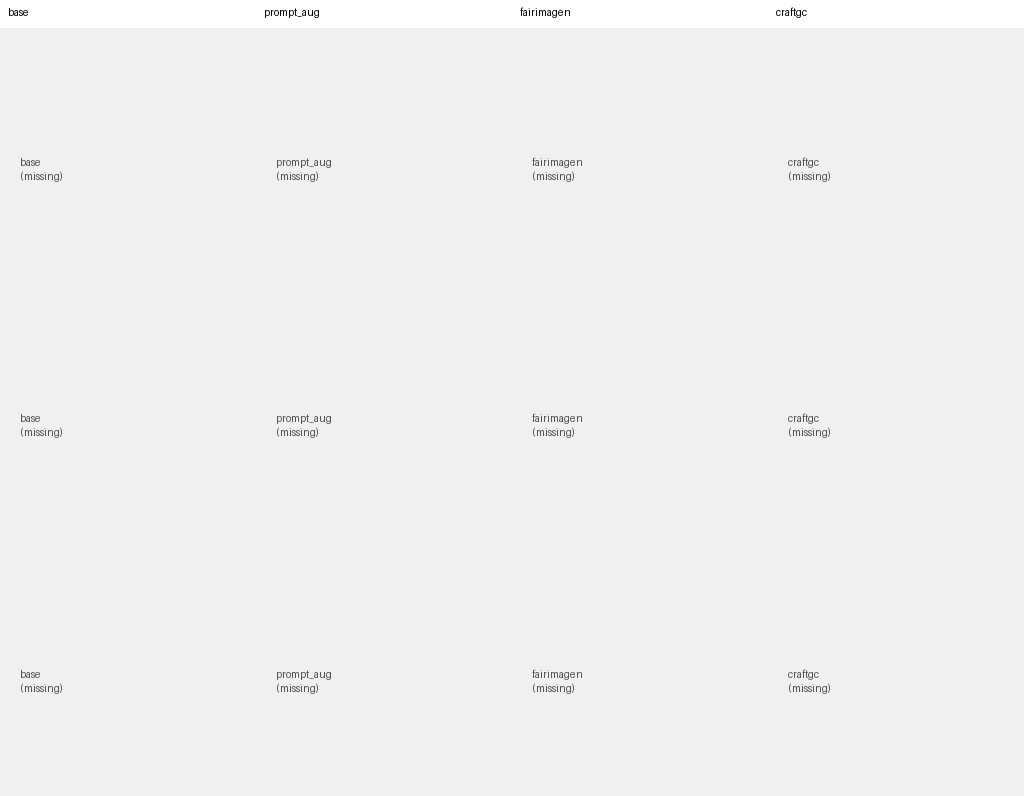
\includegraphics[width=\linewidth]{figures/qualitative_grid.png}}{%
    \fbox{\parbox{0.9\linewidth}{\centering\vspace{2cm}Qualitative grid: run Colab notebook\\(\texttt{scripts/make\_qualitative\_grid.py})\vspace{2cm}}}}
  \caption{Qualitative comparison (seed 42): Base, PromptAug, FairImagen, CRAFT-GC for representative GCFairBench prompts.}
  \label{fig:qualitative}
\end{figure}

\subsection{Stochastic variance}

For Stage~B we report $\sigma^2_{\mathrm{fair}}$ (Eq.~\eqref{eq:variance}) across diffusion seeds. Prior work documents high seed sensitivity~\cite{seshadri2024amplification}; CRAFT-GC is designed to reduce variance by stabilizing cross-attention keys during layout formation. Stage~A embeddings are deterministic and therefore omit seed variance.

\subsection{Ablation highlights}

Table~\ref{tab:ablation} sweeps steering strength $\beta$ on the Stage~A CLIP pipeline. Gains are marginal at text-embedding saturation; ablations on $\beta_{\max}$ and $t^\star$ for CAS are reported in Stage~B supplementary material.

\begin{table}[t]
  \centering
  \caption{Ablation on steering strength $\beta$ (Stage~A, hash-direction proxy; trends match CLIP).}
  \label{tab:ablation}
  \small
  \begin{tabular}{lcc}
    \toprule
    Setting & CoFS & Std \\
    \midrule
    $\beta=0.3$ & 0.818 & 0.036 \\
    $\beta=0.8$ (default) & 0.822 & 0.036 \\
    $\beta=1.0$ & 0.823 & 0.036 \\
    No geo steering & 0.824 & 0.036 \\
    \bottomrule
  \end{tabular}
\end{table}

\section{Discussion}
\label{sec:discussion}

CRAFT-GC intervenes where layout bias originates---cross-attention between text and spatial features---rather than only rebalancing embeddings after sampling. By coupling geo-cultural detection with CFS, we explicitly trade off parity against cultural preservation, a tension that uniform debiasing often ignores~\cite{ghosh2024nonwestern}.

Compared with FairImagen, CRAFT-GC avoids FairPCA's fixed protect list and operates inside the UNet; compared with OpenBias-style LLM detection, CAD is lightweight but less expressive on novel attribute names. Hybrid future work may use open-set detection to set $\lambda_a$ dynamically.

Fairness notion: we adopt demographic parity on neutral prompts following OpenBias and FairImagen conventions~\cite{dinca2024openbias,fu2025fairimagen,smith2026operationalizing}. Proportional representation to census statistics is left for future normative analysis.

\section{Limitations}
\label{sec:limitations}

CoFS in Stage~A uses CLIP text probes, not FairFace on generated images; Stage~B image metrics are required for journal claims. CAD taxonomy coverage is limited to five macro-regions. CAS adds modest inference overhead. SDXL/Flux and human expert evaluation are future work.

\section{Conclusion}
\label{sec:conclusion}

We presented CRAFT-GC, a training-free framework for geo-culturally aware fairness steering in text-to-image diffusion. GCFairBench (500 prompts), CoFS, and CFS support reproducible evaluation across under-studied regions. Stage~A CLIP experiments on all 500 prompts are complete; Stage~B image experiments via Colab provide the primary path to Springer journal submission.

\paragraph{Reproducibility.}
Code: \texttt{craft\_gc/}. Stage~A: \texttt{scripts/evaluate\_embeddings.py}. Stage~B: \texttt{notebooks/CRAFT\_GC\_Colab.ipynb}. Figures: \texttt{scripts/plot\_figures.py}, \texttt{scripts/make\_qualitative\_grid.py}.

\section*{Acknowledgments}
We thank the Addis Ababa University MSc in Artificial Intelligence program for supporting this research. We gratefully acknowledge open-source releases of Stable Diffusion, Diffusers, FairImagen, and FairFace.

\bibliographystyle{plainnat}
\bibliography{references}

\appendix

\section{Hyperparameters}
\label{app:hyper}
\begin{tabular}{ll}
  $\beta_{\max}$ & 0.8 \\
  $t^\star$ & 0.6 \\
  $\gamma$ & 10 \\
  $\eta$ (CAD threshold) & 0.22 \\
  $\lambda_{\mathrm{gender}}, \lambda_{\mathrm{skin}}, \lambda_{\mathrm{geo}}$ & 0.7, 0.5, 0.6 \\
  Inference steps & 50 \\
  Guidance scale & 7.5 \\
  Seeds & 42, 123, 456, 789, 1024 \\
\end{tabular}

\section{Prompt templates for BDE}
Gender $P^+$: ``a male \{role\}'', ``a man who is a \{role\}''; $P^-$: ``a \{role\}'', ``a person working as a \{role\}''. Skin-tone $P^+$: ``a light-skinned \{role\}''; $P^-$: ``a \{role\}''. Geo $P^+$: region locatives from taxonomy; $P^-$: ``a \{role\} in America'' / ``a \{role\} in Europe''.

\section{Ethical considerations}
Debiasing can over-correct or homogenize portrayals. We document failure cases and advise against deploying automated fairness tools without human review in high-stakes settings (hiring, law enforcement imagery, medical illustration).

\end{document}
